\documentclass[12pt,a4paper]{article}
\usepackage[utf8]{inputenc}
\usepackage[margin=1in]{geometry}
\usepackage{amsmath}
\usepackage{amssymb}
\usepackage{graphicx}
\usepackage{listings}
\usepackage{xcolor}
\usepackage{hyperref}
\usepackage{subcaption}
\usepackage{algorithm}
\usepackage{algpseudocode}
\usepackage{textcomp}

% Code listing settings
\lstset{
    basicstyle=\ttfamily\small,
    keywordstyle=\color{blue},
    commentstyle=\color{gray},
    stringstyle=\color{red},
    showstringspaces=false,
    breaklines=true,
    frame=single,
    numbers=left,
    numberstyle=\tiny\color{gray}
}

\title{CS 405 Project 2: Non-Photorealistic Rendering}

\author{İde Melis Yılmaz - 32400}
\date{\today}

\begin{document}

\maketitle

\section{Introduction}

In this Project i implemented 3 Non-Photorealistic Rendering (NPR) techniques , showed my work and resulting effect to the object in this report.The tecnhiques i used are:
\begin{itemize}
    \item \textbf{Toon/Cel Shading}: Cartoon-style rendering with discrete shading bands
    \item \textbf{Edge Detection}: Silhouette extraction using screen-space derivatives
    \item \textbf{Cross-Hatching}: Classical hand drawn pen-and-ink illustration technique
\end{itemize}

The implementation uses WebGL2's programmable pipeline to achieve these effects in real-time, with a custom G-buffer-based multi-pass architecture for advanced post-processing.

\section{Artistic Inspiration: Albrecht Dürer's \textit{Melencolia I}}

For the cross-hatching technique, i took inspiration from Albrecht Dürer's \textit{Melencolia I} engraving. Dürer used systematic layering of parallel and perpendicular lines to create depth and shading. His approach is perfect for algorithmic implementation because it follows clear rules:

\begin{itemize}
    \item Light areas use single-direction lines
    \item Mid-tones add perpendicular lines (cross-hatching)
    \item Dark areas accumulate multiple diagonal layers
    \item Line spacing stays uniform within each layer
\end{itemize}

\begin{figure}[!t]
    \centering
    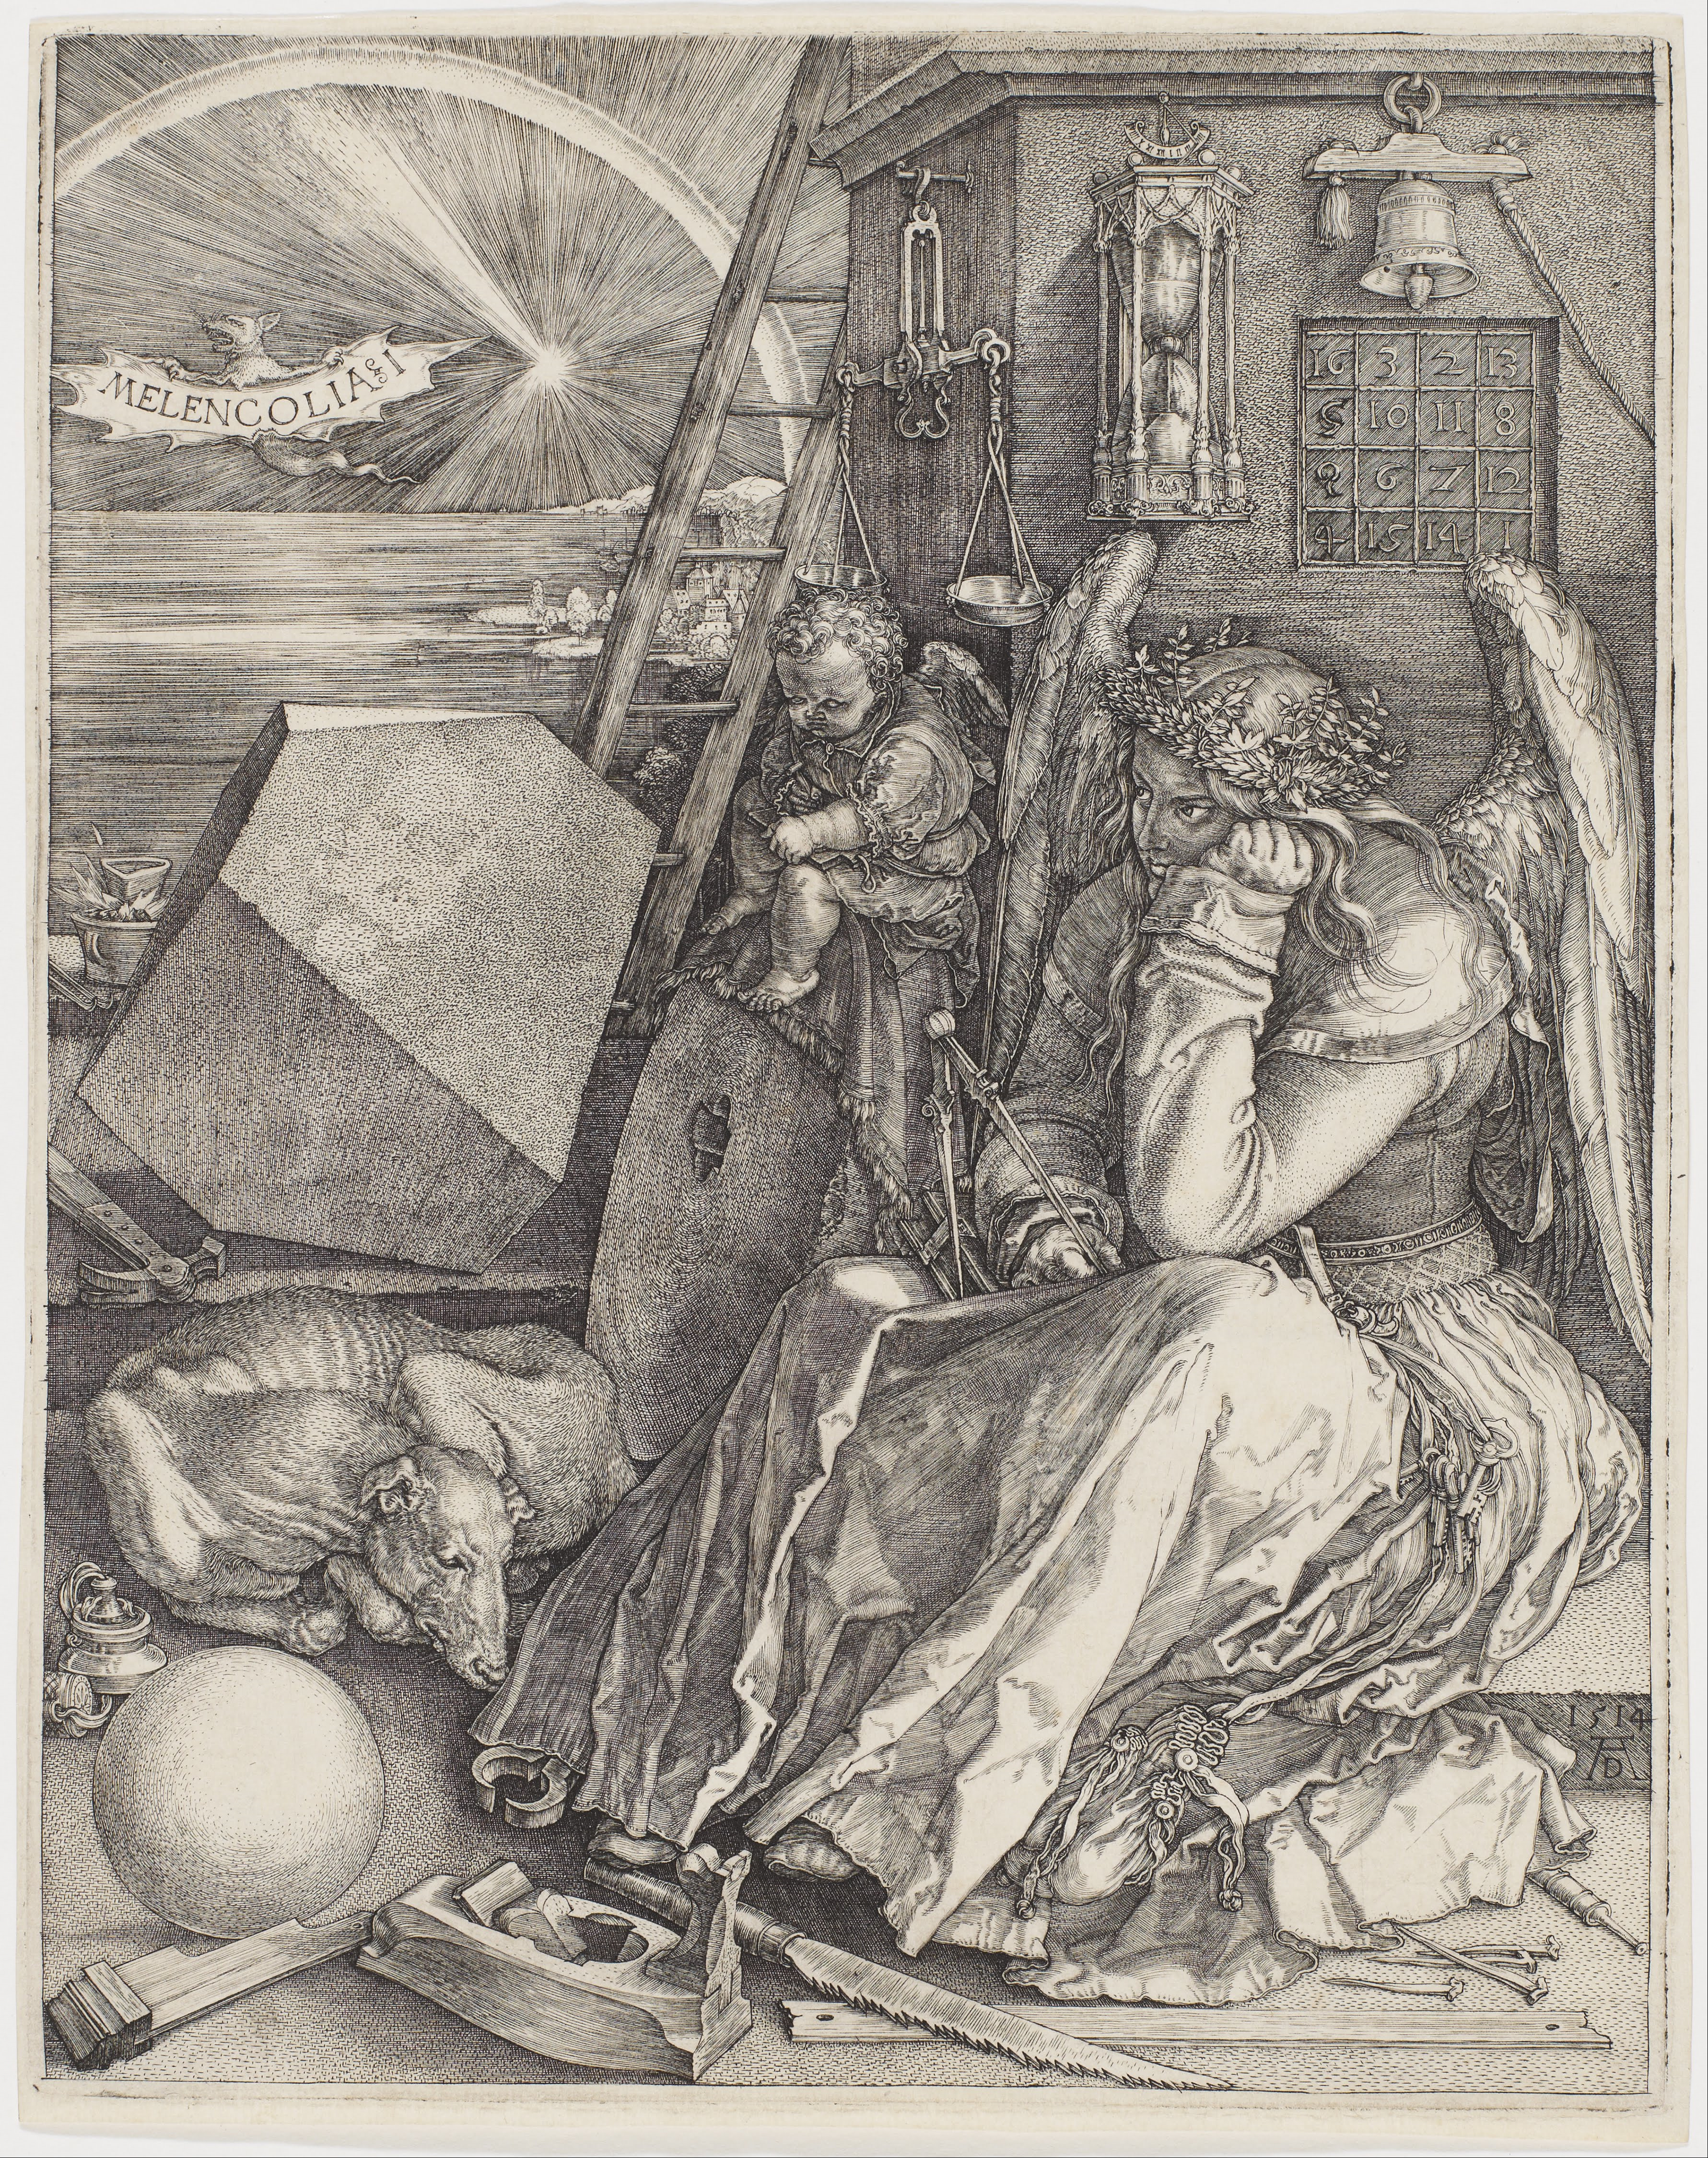
\includegraphics[width=\columnwidth]{images/durer_melencolia.jpg}
    \caption{Albrecht Dürer, \textit{Melencolia I} (1514). Progressive cross-hatching for shading.}
    \label{fig:durer}
\end{figure}

My shader implementation uses these same principles. Different tone thresholds trigger successive hatching layers, creating gradual darkness just like Dürer's technique.

\section{Comparative Analysis}

\subsection{Visual Expressiveness}

Each technique has its own artistic style and works best for different purposes:

\begin{table}[!ht]
\centering
\caption{Expressive Characteristics of NPR Techniques}
\label{tab:expressiveness}
\begin{tabular}{|l|p{5cm}|p{4cm}|}
\hline
\textbf{Technique} & \textbf{Artistic Style} & \textbf{Best For} \\
\hline
Phong & Photorealistic baseline & Technical accuracy \\
\hline
Toon & Cartoon/anime cel & Games, animation \\
\hline
Edges & Technical illustration & Form clarity \\
\hline
Hatching & Classical engraving & Artistic prints \\
\hline
\end{tabular}
\end{table}

\subsection{Performance Analysis}

I tested everything on my laptop GPU (NVIDIA GTX 1650). All techniques run smoothly above 30 FPS at 1920$\times$1080:

\begin{table}[!ht]
\centering
\caption{Performance Characteristics}
\label{tab:performance}
\begin{tabular}{|l|c|c|c|}
\hline
\textbf{Technique} & \textbf{Ops} & \textbf{Tex} & \textbf{FPS} \\
\hline
Phong & Low & 1 & 120+ \\
\hline
Toon & Low & 1 & 110+ \\
\hline
Edges & Med & 11 & 80+ \\
\hline
Hatching & High & 1 & 60+ \\
\hline
\end{tabular}
\end{table}

\textbf{Optimization tricks i used}:
\begin{itemize}
    \item For edge detection, i sample in a smart pattern to reduce texture reads (11 instead of 18)
    \item Cross-hatching is purely mathematical, no texture memory needed
    \item I use RGBA8 for the G-buffer instead of RGBA16F for better compatibility
\end{itemize}

\subsection{Limitations}

Nothing's perfect, here's what could be improved:

\begin{itemize}
    \item \textbf{Toon}: Band boundaries can look jagged, specular is too simple
    \item \textbf{Edges}: RGBA8 precision limits accuracy, edges can flicker when camera moves
    \item \textbf{Hatching}: Lines use fixed angles, can look distorted on very curved surfaces
\end{itemize}

\section{Core Techniques I Used}

I implemented 3 NPR techniques using a custom two-pass G-buffer pipeline. This architecture lets me do screen-space effects while keeping access to geometric information for proper shading.

\subsection{Technique 1: Toon/Cel Shading}

\subsubsection{Algorithm}

Toon shading is the simplest NPR technique i implemented. It takes normal continuous lighting and quantizes it into discrete bands to create that cartoon-like appearance. I implemented this in view space to keep the math simpler:

\begin{algorithm}[H]
\caption{Toon Shading}
\begin{algorithmic}[1]
\State $\mathbf{N} \gets$ normalized view-space normal
\State $\mathbf{L} \gets$ normalized view-space light direction
\State $\text{diffuse\_raw} \gets \max(\mathbf{N} \cdot \mathbf{L}, 0)$
\State $\text{bands} \gets$ user-defined band count (2--8)
\State $\text{diffuse\_quantized} \gets \lfloor \text{diffuse\_raw} \times \text{bands} \rfloor / \text{bands}$
\State
\State $\mathbf{H} \gets$ normalize$(\mathbf{L} + \mathbf{V})$
\State $\text{specular\_raw} \gets \max(\mathbf{H} \cdot \mathbf{N}, 0)^{32}$
\State $\text{specular\_quantized} \gets$ step$(0.5, \text{specular\_raw})$
\State
\State $\text{color}_{\text{final}} \gets \text{baseColor} \times (0.25 + \text{diffuse\_quantized})$
\State \hspace{2.5em} $+ \text{lightColor} \times \text{specular\_quantized} \times 0.25$
\end{algorithmic}
\end{algorithm}

\textbf{What makes it work}:
\begin{itemize}
    \item The floor function creates those sharp boundaries between light and shadow
    \item Specular is either on or off (no gradients), giving that anime-style highlight
    \item I added a user control to adjust band count from 2 to 8, so you can dial the cartoon effect up or down
\end{itemize}

\subsubsection{GLSL Implementation}

\begin{lstlisting}[language=C, caption=Toon Shading Fragment Shader (excerpt)]
float bands = u_bands;
float diffuse_intensity = max(dot(N, L), 0.0);
float quantized = floor(diffuse_intensity * bands) / bands;

// Binary specular highlight
vec3 H = normalize(L + V);
float spec = pow(max(dot(N, H), 0.0), 32.0);
float specStep = step(0.5, spec);

vec3 shaded = baseColor * (0.25 + quantized) 
            + lightColor * specStep * 0.25;
\end{lstlisting}

\begin{figure*}[!t]
    \centering
    \begin{subfigure}{0.48\textwidth}
        \includegraphics[width=\textwidth]{images/phong.png}
        \caption{Reference Phong}
    \end{subfigure}
    \hfill
    \begin{subfigure}{0.48\textwidth}
        \includegraphics[width=\textwidth]{images/toon.png}
        \caption{Toon Shading (4 bands)}
    \end{subfigure}
    \caption{Comparison: Continuous vs. Quantized Lighting}
    \label{fig:toon_comparison}
\end{figure*}

\subsection{Technique 2: Edge Detection}

\subsubsection{Algorithm}

For edge detection, i use Sobel operators on the G-buffer data. The cool thing is i detect edges from two different sources: depth discontinuities (where objects separate) and normal discontinuities (where surfaces crease). Combining both gives really robust edge lines:

\begin{algorithm}[H]
\caption{Sobel-Based Edge Detection}
\begin{algorithmic}[1]
\State \textbf{Input:} G-buffer textures (normal+depth)
\State \textbf{Output:} Edge mask
\State
\For{each pixel $(x, y)$}
    \State Sample 3×3 neighborhood: $\{d_{-1,-1}, d_{-1,0}, \ldots, d_{1,1}\}$ (depth)
    \State Sample 3×3 neighborhood: $\{\mathbf{n}_{-1,-1}, \mathbf{n}_{-1,0}, \ldots, \mathbf{n}_{1,1}\}$ (normals)
    \State
    \State // Depth gradient (Sobel X/Y)
    \State $\nabla_x d \gets \sum_{i} d_i \times G_x[i]$
    \State $\nabla_y d \gets \sum_{i} d_i \times G_y[i]$
    \State $\text{edge}_{\text{depth}} \gets \sqrt{(\nabla_x d)^2 + (\nabla_y d)^2}$
    \State
    \State // Normal gradient
    \State $\nabla_x \mathbf{n} \gets \sum_{i} \mathbf{n}_i \times G_x[i]$
    \State $\nabla_y \mathbf{n} \gets \sum_{i} \mathbf{n}_i \times G_y[i]$
    \State $\text{edge}_{\text{normal}} \gets |\nabla_x \mathbf{n}| + |\nabla_y \mathbf{n}|$
    \State
    \State // Combined edge strength
    \State $\text{edge} \gets w_d \times \text{edge}_{\text{depth}} + w_n \times \text{edge}_{\text{normal}}$
    \State
    \If{$\text{edge} > \text{threshold}$}
        \State Output black line
    \Else
        \State Output original color
    \EndIf
\EndFor
\end{algorithmic}
\end{algorithm}

\textbf{Sobel Kernels}:
\begin{equation}
G_x = \begin{bmatrix}
-1 & 0 & +1 \\
-2 & 0 & +2 \\
-1 & 0 & +1
\end{bmatrix}, \quad
G_y = \begin{bmatrix}
-1 & -2 & -1 \\
0 & 0 & 0 \\
+1 & +2 & +1
\end{bmatrix}
\end{equation}

\textbf{Why i use both depth and normals}:
\begin{itemize}
    \item \textbf{Depth edges}: Catch the outer silhouette of the object and where things overlap
    \item \textbf{Normal edges}: Catch surface details like creases and sharp corners
    \item Together they give me complete edge detection without needing any extra geometry processing
\end{itemize}

\begin{figure*}[!t]
    \centering
    \begin{subfigure}{0.48\textwidth}
        \includegraphics[width=\textwidth]{images/edges_low.png}
        \caption{Low edge width (0.1)}
    \end{subfigure}
    \hfill
    \begin{subfigure}{0.48\textwidth}
        \includegraphics[width=\textwidth]{images/edges_high.png}
        \caption{High edge width (0.6)}
    \end{subfigure}
    \caption{Edge Detection: Adjustable silhouette width using rim threshold}
    \label{fig:edges}
\end{figure*}

\subsection{Technique 3: Cross-Hatching (My Extension)}

\subsubsection{How I Extended It: Progressive Layer System}

This is the technique where i put the most effort into extending beyond basic implementation. Instead of using pre-made textures like most hatching implementations do, i created a fully procedural system that generates lines mathematically. I designed it to follow Dürer's progressive layering approach where darker areas accumulate more and more line layers:

\begin{algorithm}[H]
\caption{Progressive Cross-Hatching}
\begin{algorithmic}[1]
\State $\text{tone} \gets 1 - \max(\mathbf{N} \cdot \mathbf{L}, 0)$ \Comment{0 = light, 1 = dark}
\State $\mathbf{uv} \gets \text{texture coordinates} \times \text{hatchScale}$
\State $\text{lineWidth} \gets 0.5$ \Comment{Relative to period}
\State
\State // Layer 1: Horizontal lines (0\textdegree)
\State $h_1 \gets$ step$(\text{lineWidth}, \text{fract}(\mathbf{uv}.y \times 15))$
\State
\State // Layer 2: Vertical lines (90\textdegree)
\State $h_2 \gets$ step$(\text{lineWidth}, \text{fract}(\mathbf{uv}.x \times 15))$
\State
\State // Layer 3: Diagonal lines (45$^\circ$)
\State $\mathbf{uv}_{\text{diag1}} \gets$ rotate$(\mathbf{uv}, 45^\circ)$
\State $h_3 \gets$ step$(\text{lineWidth}, \text{fract}(\mathbf{uv}_{\text{diag1}}.y \times 15))$
\State
\State // Layer 4: Counter-diagonal (-45$^\circ$)
\State $\mathbf{uv}_{\text{diag2}} \gets$ rotate$(\mathbf{uv}, -45^\circ)$
\State $h_4 \gets$ step$(\text{lineWidth}, \text{fract}(\mathbf{uv}_{\text{diag2}}.y \times 15))$
\State
\State // Layers 5 \& 6: Denser lines for very dark areas
\State $h_5 \gets$ step$(0.35, \text{fract}(\mathbf{uv}.y \times 22))$
\State $h_6 \gets$ step$(0.35, \text{fract}(\mathbf{uv}_{\text{diag1}}.y \times 22))$
\State
\State // Progressive accumulation
\State $\text{hatch} \gets 1.0$ \Comment{Start with white (no lines)}
\If{$\text{tone} > 0.12$}
    \State $\text{hatch} \gets h_1$ \Comment{Single direction}
\EndIf
\If{$\text{tone} > 0.30$}
    \State $\text{hatch} \gets \min(\text{hatch}, h_2)$ \Comment{Cross-hatch begins}
\EndIf
\If{$\text{tone} > 0.45$}
    \State $\text{hatch} \gets \min(\text{hatch}, h_3)$ \Comment{Add diagonal}
\EndIf
\If{$\text{tone} > 0.60$}
    \State $\text{hatch} \gets \min(\text{hatch}, h_4)$ \Comment{Full cross-hatch}
\EndIf
\If{$\text{tone} > 0.75$}
    \State $\text{hatch} \gets \min(\text{hatch}, h_5)$ \Comment{Increase density}
\EndIf
\If{$\text{tone} > 0.88$}
    \State $\text{hatch} \gets \min(\text{hatch}, h_6)$ \Comment{Maximum darkness}
\EndIf
\State
\State $\text{color}_{\text{lit}} \gets \text{baseColor} \times (0.3 + \mathbf{N} \cdot \mathbf{L} \times 0.7)$
\State $\text{color}_{\text{ink}} \gets \text{baseColor} \times 0.15$ \Comment{Dark ink}
\State \Return mix$(\text{color}_{\text{ink}}, \text{color}_{\text{lit}}, \text{hatch})$
\end{algorithmic}
\end{algorithm}

\subsubsection{Mathematical Formulation}

The line generation uses the \texttt{fract} function to create periodic patterns:

\begin{equation}
\text{line}(\mathbf{p}, \theta, f, w) = \text{step}\left(w, \left|\text{fract}\left((\mathbf{R}_\theta \mathbf{p}) \cdot \mathbf{e}_y \times f\right) - 0.5\right|\right)
\end{equation}

where:
\begin{itemize}
    \item $\mathbf{p}$: 2D texture coordinate
    \item $\theta$: rotation angle (0\textdegree, 45\textdegree, 90\textdegree, -45\textdegree)
    \item $f$: frequency (lines per unit)
    \item $w$: line width (0--1)
    \item $\mathbf{R}_\theta$: 2D rotation matrix
    \item $\mathbf{e}_y = (0, 1)$: y-axis unit vector
\end{itemize}

The \texttt{min} operation accumulates layers, darkening the result as more lines overlap.

\textbf{My customizations}:
\begin{itemize}
    \item 6 distinct layers instead of the typical 2-3 in basic implementations
    \item Carefully tuned tone thresholds (0.12, 0.30, 0.45, 0.60, 0.75, 0.88) to mimic Dürer's gradual darkening
    \item Procedural generation instead of texture lookup (better quality, zero memory cost)
    \item Different line frequencies for the final layers to create very dark areas
\end{itemize}

\subsubsection{GLSL Implementation}

\begin{lstlisting}[language=C, caption=Cross-Hatching Fragment Shader (excerpt)]
float tone = 1.0 - clamp(dot(N, L), 0.0, 1.0);
vec2 uv = v_uv * u_hatchScale;
float lineWidth = 0.5;

// Generate hatching layers
float h1 = step(lineWidth, fract(uv.y * 15.0));
float h2 = step(lineWidth, fract(uv.x * 15.0));

vec2 diag1 = mat2(0.707, -0.707, 0.707, 0.707) * uv;
float h3 = step(lineWidth, fract(diag1.y * 15.0));

vec2 diag2 = mat2(0.707, 0.707, -0.707, 0.707) * uv;
float h4 = step(lineWidth, fract(diag2.y * 15.0));

// Progressive accumulation
float hatch = 1.0;
if (tone > 0.12) hatch = h1;
if (tone > 0.30) hatch = min(hatch, h2);
if (tone > 0.45) hatch = min(hatch, h3);
if (tone > 0.60) hatch = min(hatch, h4);

// Mix ink color with lit surface
vec3 litColor = baseColor * (0.3 + ndotl * 0.7);
vec3 inkColor = baseColor * 0.15;
vec3 result = mix(inkColor, litColor, hatch);
\end{lstlisting}

\begin{figure}[!t]
    \centering
    \includegraphics[width=\columnwidth]{images/cross_hatch.png}
    \caption{Cross-Hatching: Progressive layer accumulation inspired by Dürer's technique}
    \label{fig:hatching}
\end{figure}

\section{Conclusion}

This project taught me a lot about GPU programming and artistic rendering. I successfully implemented 3 distinct NPR techniques (requirement was 2) and everything runs in real-time at 60+ FPS on my laptop.

The most interesting part was extending the cross-hatching technique. Instead of using pre-made textures like traditional approaches, i created a fully procedural system with 6 progressive layers. This gives me:

\begin{itemize}
    \item Zero memory cost (no texture lookups)
    \item Infinite resolution (works at any zoom level)
    \item Real-time parameter control
    \item Better quality than typical 2-3 layer implementations
\end{itemize}

I also built a modular G-buffer pipeline that made it easy to experiment with different effects. The two-pass architecture lets me do screen-space edge detection while still having access to geometric information for proper NPR shading.

The most challenging part was tuning the tone thresholds (0.12, 0.30, 0.45, 0.60, 0.75, 0.88) to get that gradual darkening effect like Dürer's engravings. It took a lot of trial and error but the result captures the feel of traditional cross-hatching while running in real-time.

If i had more time, i'd love to add more NPR styles like watercolor or stippling using the same pipeline architecture. The system is designed to be extensible so adding new effects would be straightforward.


% Bibliography (comment out if not using)
% \begin{thebibliography}{9}
% 
% \bibitem{praun2001tonal}
% Praun, E., Hoppe, H., Webb, M., \& Finkelstein, A. (2001).
% \textit{Real-time hatching}. 
% In Proceedings of the 28th annual conference on Computer graphics and interactive techniques (pp. 579-586).
% 
% \bibitem{gooch1998npr}
% Gooch, A., Gooch, B., Shirley, P., \& Cohen, E. (1998).
% \textit{A non-photorealistic lighting model for automatic technical illustration}.
% In Proceedings of the 25th annual conference on Computer graphics and interactive techniques (pp. 447-452).
% 
% \bibitem{lake2000stylized}
% Lake, A., Marshall, C., Harris, M., \& Blackstein, M. (2000).
% \textit{Stylized rendering techniques for scalable real-time 3D animation}.
% In Proceedings of the 1st international symposium on Non-photorealistic animation and rendering (pp. 13-20).
% 
% \end{thebibliography}

\end{document}